\documentclass[]{final_report}
\usepackage{graphicx}
\usepackage{hyperref}
\usepackage{titlesec}
\usepackage[utf8]{inputenc}
\usepackage[backend=biber, style=ieee]{biblatex}
\usepackage{amsmath}
\usepackage{amssymb}
\usepackage{float}
\usepackage{tabularx} % Needed for the X column type
\usepackage{booktabs} % For prettier tables
\usepackage{lipsum}   % For dummy text
\usepackage{mathtools}
\usepackage{stmaryrd}
\usepackage{mdframed}
\usepackage{caption}
\usepackage{array}
\usepackage{listings}
\usepackage{xcolor}  % for custom colors
\usepackage{adjustbox}
\usepackage{tikz}
\usepackage{rotating}
\usepackage{pdflscape}
\usepackage{fancyhdr}

\fancypagestyle{lscape}{%
  \fancyhf{} % clear all header and footer fields
  \fancyfoot[LE,RO]{\makebox[0pt][l]{\rotatebox[origin=c]{90}{\thepage}}} % Left Even, Right Odd
  \renewcommand{\headrulewidth}{0pt}
  \renewcommand{\footrulewidth}{0pt}
}


\addbibresource{fyp.bib}
\usepackage{amsthm}
\theoremstyle{definition}
\newtheorem{definition}{Definition}[chapter]
\newtheorem{basic}{Basic Definition}

% Define the Java code style
\lstdefinestyle{mystyle}{
    language=Java,
    commentstyle=\color{green},
    keywordstyle=\color{blue},
    numberstyle=\tiny\color{gray},
    stringstyle=\color{red},
    basicstyle=\ttfamily\footnotesize,
    breakatwhitespace=false,         
    breaklines=true,                 
    captionpos=b,                    
    keepspaces=true,                 
    numbers=left,                    
    numbersep=5pt,                  
    showspaces=false,                
    showstringspaces=false,
    showtabs=false,                  
    tabsize=2
}
\lstset{style=mystyle}


%%%%%%%%%%%%%%%%%%%%%%
%%% Input project details
\def\studentname{Jude Asare}
\def\reportyear{2023/2024}
\def\projecttitle{Implementing the PKCS\#1 v1.5 Signature Scheme with provably secure parameters}
\def\supervisorname{Saqib Kakvi}
\def\degree{MSci (Hons) in Computer Science (Information Security)}
\def\fullOrHalfUnit{MSci} 
\def\finalOrInterim{Interim Report} 
\begin{document}

\maketitle





%%%%%%%%%%%%%%%%%%%%%%
%%% Table of Contents
\tableofcontents\pdfbookmark[0]{Table of Contents}{toc}\newpage



%%%%%%%%%%%%%%%%%%%%%%
%%% Your Abstract here

\begin{abstract}



The PKCS\#1 v1.5 digital signature scheme has been widely utilised in protocols such as SSH, DNSSEC, IKE, and most prominently, in TLS up to version 1.2. Since its inception in 1998 \cite{rfc2313} it has played a pivotal role in the landscape of digital security comprising the most widely used digital signature scheme in practice. The scheme, renowned for its straightforwardness and expedited verification capabilities, has seen persistent integration across diverse cryptographic systems. 

Nevertheless, amidst its widespread acceptance, it's been marred by several challenges. Among these are the targeting of a latent vulnerability with incorrectly implemented signature verification implementations \cite{finney2006bleichenbacher, kuhn2008variants, bock2018return} stemming from attacks \cite{bleichenbacher1998chosen} exploiting its provably insecure associated encryption paradigm \cite{rfc2313} and a glaring absence of a rigorous security proof that validates its robustness.

Even though alternatives like RSA-PSS offer provable security (\cite{bellare1996exact}, \cite{jonsson2001security}), they come with inherent problem, such as the introduction of randomness and a hike in computational complexity. These issues have created reservations for its wholesale adoption in place of PKCS\#1 v1.5 e.g., RSA-PSS and was only upgraded to a requirement for new applications in PKCS\#1 v2.2 \cite{rfc8017} long after initially being suggested as the replacement for PKCS\#1 v1.5 in PKCS\#1 v2.1 \cite{rfc3447}. Imperative requirements of backward compatibility and interoperability have been the main detractors of the aversion to replacing PKCS\#1 v1.5 and while RSA-PSS is now required in new applications, they entail retaining PKCS\#1 v1.5 in some form at the very least, as a preferable choice.
 
A significant breakthrough came in 2018 when Jager, Kakvi, and May \cite{jager2018security} provided a security proof for the PKCS\#1 v1.5 Signature scheme building on the work of Coron \cite{coron2002security}. Although still requiring the adoption of larger cryptographic parameters deviating slightly from standard use, their methods were flexible enough to show instantiations in practice such that the improved proofs apply. Benefits not limited to PKCS\#1 v1.5, their work also offered insights enabling the proof to apply to other deterministic RSA signature schemes, with similar construction patterns including ISO/IEC 9796-2 and ANSI X9.31 schemes.

Guided by this revelation, this project seeks to concretely implement these signature schemes, with a primary emphasis on the PKCS\#1 v1.5 signature scheme, using the aforementioned provably secure parameters. This project primarily aims to dissect the computational burdens these parameters introduce into deterministic RSA schemes. This aim is supplemented by supporting objectives to produce algorithms that facilitate its implementation with provably secure parameters and standard parameters. From there the main objective is to produce a user-interfaced benchmarking program to explore aforementioned overhead across standards. 
\newpage
\end{abstract}
\newpage


%%%%%%%%%%%%%%%%%%%%%%
%%% Introduction
\chapter{Introduction}


\section{Aims}

\subsection{Why: The Context and Rationale}
The PKCS\#1 v1.5 digital signature scheme, rooted in RSA's hash-and-sign framework, has emerged as the de facto standard for digital signatures since its 1998 introduction \cite{rfc2313}. Essential in security-focused network protocols like SSH, DNSSEC, IKE, and pre-TLS 1.3 X.509 certificates \cite{schaad2005additional}, its simplicity fostered broad adoption from its outset with a straightforward implementation across programming languages, and speedy verifications relative to alternatives like DSA or ECDS  \cite{jager2018security}. 
Despite its widespread adoption the scheme lacks formal security proofs, raising concerns about its long-term reliability.
Given its deep integration in various applications, even at the hardware level, transitioning to provably secure alternatives like RSA-PSS has been slow (RSA-PSS (\cite{bellare1996exact}, \cite{jonsson2001security}) only upgraded to a requirement for new applications in PKCS\#1 v2.2 \cite{rfc8017} long after initially being suggested as the replacement for PKCS\#1 v1.5 in PKCS\#1 v2.1 \cite{rfc3447}).

Additionally considered in a broader sense, for  a cryptographic scheme i.e., RSA-PSS to gain traction, it has to be developed, vetted by experts, standardised at both primitive and protocol levels, implemented in software accordingly, and then set as default. RSA-PSS, while superior to the older PKCS\#1 v1.5, lingers in the later stages of this transition between implementation in software and being set as the default in applications. This means retaining PKCS\#1 v1.5 scheme remains a preferable choice considering the state of the art.

A landmark development came in 2018 when Jager, Kakvi, and May \cite{jager2018security} provided a security proof (an improvement on Coron \cite{coron2002security} proof that was limited to the Rabin-Williams variant with e=2) for the PKCS\#1 v1.5 signature scheme but only if larger parameters are used. Their work offered insights that also apply to other deterministic RSA signature schemes, including ISO/IEC 9796-2 Scheme and ANSI X9.31.

\subsection{What: The Primary Goal}
The aim of this project was to bridge the theoretical insights presented by the authors \cite{jager2018security} with practical implementation, subsequently evaluating the computational overhead induced by the application of provably secure parameters to deterministic RSA schemes, with a particular focus on the PKCS standard. 

\subsection{How: Overview of Objectives}
The influence of the application of provably secure parameters to each of the mentioned deterministic schemes in terms of computational cost was investigated. This was done through the production of algorithms respective to both cases (standard and provably secure parameters) allowing for comparison. Performing the investigation across standards was means of ascertaining a more reliable and accurate assessment by enabling further comparison of introduced overhead across different schemes. The final deliverable constituted an all-incorporative user-interfaced benchmarking program for which results from automation of signature processes applied to data were generated for appropriate evaluations and conclusions to be drawn.


\section{Objectives}
To achieve the aim, the project will involve:
\begin{itemize}
    \item Develop concrete implementations of the PKCS\#1 v1.5 signature schemes using both standard and provably secure parameters.
    \item Develop concrete implementations of  the ISO/IEC 9796-2 Scheme, and separately the ANSI X9.31 signature schemes using both standard and provably secure parameters.
    \item Demonstrate in practice, with larger parameters, how deterministic schemes, particularly the PKCS\#1 v1.5 signature scheme  can achieve a security level on par with less-practical, signature schemes, such as RSA-PSS.
    \item Create a user-interfaced benchmarking program that incorporates all objectives of the project to assess this overhead in various scenarios across standards
\end{itemize}



 
\chapter{Literature Review/Related Work}
RSASSA-PKCS1-v1.5 remains unbroken. There are no real attacks able to successfully exploit the scheme free of implementation errors. This distinction of being free of implementation errors is crucial. Potential proofs consider only forgeries that are accepted by a correct verification algorithm. It is now well established from a variety of follow up studies all originating from \cite{bleichenbacher1998chosen} that vulnerable implementations of a flawed signature verification algorithm for RSASSA-PKCS1-v1.5 can be exploited. Bleichenbacher presented a low-exponent attack on RSA-PKCS\#1 v1.5 signatures at the CRYPTO 2006 rump session. This attack was later described by Finney \cite{finney2006bleichenbacher} in a posting to the OpenPGP mailing list. 

It was not until the efforts of Coron \cite{coron2002security} in 2002 that a security proof applicable to RSASSA-PKCS1-v1.5 arrived. This was due to the issue of deterministic padding scheme that RSASSA-PKCS1-v1.5 uses rendering standard proof techniques void. Coron presented a security proof for RSASSA-PKCS1-v1.5 (and ISO/IEC 9796-2 signatures) albeit with a restriction that e = 2, i.e. the Rabin-Williams variant \cite{coron2002security} which is secure based on the factoring assumption. 
The proofs' exclusive and/or restrictive value of e aside, a further caveat was that the output size of the hash function needed to be 2/3 of the bit length of the modulus N. These restrictions diverge largely from the parameters used in the instantiation of RSA-PKCS\#1 v1.5 signatures in practice. 

Much later, Jager, Kakvi and May \cite{jager2018security} showed an improved security proof for RSASSA-PKCS1-v1 5 with less restrictive conditions.
It sufficed that e more generally be a small prime (Kakvi and Kiltz \cite{kakvi2018optimal}). Still requiring a large hash function output, Jager, Kakvi and May achieved an improvement in hash function output requiring only 1/2 of the modulus size. The modulus effectively doubles in bit length when compared to the norm with a newly introduced third prime factor necessitating the increase in bits.
Withstanding the improvement and as a consequence of the proofs being founded in the random oracle model, the larger cryptographic parameters still deviate slightly from the standard parameters used in practice. Nonetheless this was sufficient enough for the authors to demonstrate how RSA-PKCS\#1 v1.5 signatures can be instantiated in practice such that the improved proofs apply. 

To all intents and purposes, regardless of the proofs being presented primarily for RSASSA-PKCS1-v1.5, uniformity in construction philosophy means other signature standards of the same deterministic RSA type (ISO/IEC 9796-2 signatures and ANSI X9.31 rDSA) still match the setting required for proofs to be applicable to them. For example theorem statements used in construction of Corons' proof \cite{coron2002security} are general enough that corresponding proof theorems can also be presented for the remaining standards of deterministic signatures. 

A full discussion of provable security extending to non-deterministic schemes lies beyond the scope of this project. Probabilistic padding poses an issue since generating sources of randomness, particularly on constrained devices is an ongoing challenge. Moreover RSA-PSS, the sole RSA-based randomised digital signature scheme uses two hash functions. This makes it difficult to compare with deterministic schemes that use only one. This project focused on standardised deterministic schemes which are directly comparable and subversion resistant \cite{ateniese2015subversion} by default of not having to generate randomness. This lends well to the issue of examining computational overhead from various perspectives of the different deterministic standards.



\chapter{Cryptographic Foundations}
\section{Notations}
The security parameter is denoted as \( \lambda \). 
This parameter determines a system's security level/key sizes (higher values mean better security but more computational effort). For all \( n \in \mathbb{N} \), the symbol \( 1^n \) represents the n-bit string of all ones. Given any set \( S \), the notation \( x \stackrel{R}{\leftarrow} S \) signifies that \( x \) is chosen uniformly at random from \( S \).  The set of prime numbers is represented as \( \mathbb{P} \) and the set of \( k \)-bit integers is denoted as \( \mathbb{Z}[k] \). Similarly, the set of \( k \)-bit primes is indicated by \( \mathbb{P}[k] \). The notation \( \mathbb{Z}_N^* \) represents the multiplicative group modulo \( N \) where \( N \in \mathbb{N} \). Game-based proofs are employed, and the notation \( G^A \Rightarrow 1 \) indicates an event where the adversary \( A \) succeeds in game \( G \), specifically when the Finalise Procedure yields an output of 1.


\section{Digital Signature Schemes}
Not every security issue revolves around confidentiality, and adversaries are not restricted to merely passive surveillance. In numerous scenarios, safeguarding the authenticity and integrity of communications from active opponents, who might manipulate or introduce unauthorised messages into the transmission, is paramount or even more critical. In the public key setting, the cryptographic primitive used to provide data integrity is a digital signature scheme. Essentially, Digital signatures function as a means binding an identity to specific information. A signature process consists of transforming the relevant message and the entity's confidential details to produce tag named a signature. 
For instance, authors can use these to ensure their writings are received by their readers unaltered, enabling readers to confirm the content's authenticity using the distributed public key.


\begin{definition}
\label{def:digital signature}
A (digital) signature scheme consists of three probabilistic polynomial-time algorithms (Gen, Sign, Vrfy) such that:
\begin{enumerate}
    \item Gen (key-generation algorithm): takes as input a security parameter $1^\lambda$ and outputs a pair of keys $(sk ,vk)$, where $sk$ is the signing key and $vk$ is the verification key.
    \item Sign (signing algorithm): takes as input a private key $sk$ and a message $m$ and outputs a signature $\sigma$. ($\sigma \leftarrow \text{Sign}_{sk}(m)$).
    \item Vrfy (deterministic verification algorithm):  takes as input a public key $pk$, a message $m$, and a signature $\sigma$; outputs a boolean ($b := \text{Vrfy}_{pk}(m, \sigma)$).
\end{enumerate}
\end{definition}




Correctness: It is required that except with negligible probability over (pk, sk) output by Gen($1^\lambda$), it holds that $\text{Vrfy}_{pk} (m, \text{Sign}_{sk}(m)$) = 1 for every (legal) message m. 

Such a signature scheme can be utilised in the following way. 
Bob (sender) runs Gen($1^\lambda$) in turn generating the keys (pk, sk). Bob then makes his public key (pk) available to everyone, including Alice (receiver). 
When Bob wants to send a message m to Alice and ensure it's authentic, he generates a signature $\sigma$ for that message using his private key: $\sigma \leftarrow \text{Sign}_{sk}(m)$. He then sends both the message and its signature, (m, $\sigma$), to Alice.

Upon receipt of (m, $\sigma$), Alice, who already knows Bob's public key can verify the authenticity of m by checking whether $\text{Vrfy}_{pk} (m, \text{Sign}_{sk}(m)$) $\stackrel{?}{=} 1$. This assures Alice both that Bob sent m, and additionally that m was not modified in transit

\section{Security of signature schemes}
Security for a signature scheme, represented as DS = (Gen, Sign, Vrfy), is depicted through a contest between a challenger and an Adversary A (probabilistic machine operating within polynomial time). This contest emulates a situation in which A endeavours to compromise the signature scheme by employing a specific attack model. 

\subsection{Default notion of Secure Signatures}
The intuitive idea behind the default notion of security for digital signature schemes is that no efficient adversary should be able to generate valid digital signature for any "new" document that was not previously signed by the original signer.
An adversary might see all documents and their associated signatures (with aid of sign oracle) and even influence document content (Replay Attacks).

A robust digital signature system, resistant to such forgeries, is termed existentially unforgeable under an adaptive chosen-message attack. "Existentially unforgeable" signifies that the adversary cannot produce a valid signature on any document. The protection should remain intact even if the adversary can carry out an adaptive chosen-message attack by which it is able to obtain signatures on arbitrary messages chosen adaptively during its attack.

\begin{figure}[H]
\centering
\hfill Game UF-CMA(ROM)\hfill\phantom{} 
\[
\boxed{
\begin{aligned}
&\underline{\textbf{\text{Initialise}}} \\
&(pk, sk) \leftarrow_\$ \text{Gen}(1^\lambda) \\
&\text{return } pk \\
\\
&\underline{\textbf{\text{Hash}}(m)} \\
&\text{if } (m, \cdot) \in \mathcal{H} \\
&\quad \text{fetch } (m, y) \in \mathcal{H} \\
&\quad \text{return } y \\
&\text{else} \\
&\quad y \in_{R} \text{Domain}; \\
&\quad \mathcal{H} \leftarrow \mathcal{H} \cup\{(m, y)\} \\
&\quad \text{return } y \\
\\
&\underline{\textbf{\text{Sign}}(m)} \\
&\mathcal{M} \leftarrow \mathcal{M} \cup\{m\} \\
&\text{return } \sigma \leftarrow_{\$} \text{Sign}(sk, m) \\
\\
&\underline{\textbf{\text{Finalise}}(m^*, \sigma^*)} \\
&\text{if Vrfy}(pk, m^*, \sigma^*) == 1 \land m^* \notin \mathcal{M} \\
&\quad \text{return } 1 \\
&\text{else} \\
&\quad \text{return } 0
\end{aligned}
}
\]
\caption{Game defining UF-CMA security in the Random Oracle Model (section \ref{subSec:ROM}.)}
\label{fig:crypto_game}
\end{figure}
\begin{definition}
A signature scheme DS is UF-CMA secure, if for any forger $\mathcal{F}$ running in time at most $t$, making at most $q_h$ hash queries and making at most $q_s$ signature queries, we have:
\[
\textbf{Adv}_{\mathcal{F},\text{DS}}^{\text{UF-CMA}} = \Pr \left[ \begin{aligned} &1 \leftarrow \textbf{Finalise}(m^*, \sigma^*); \\ &(m^*, \sigma^*) \leftarrow \mathcal{F}^{\textbf{Hash}(\cdot),\textbf{Sign}(\cdot)}(pk); \\ &\texttt{pk} \leftarrow_{\$} \textbf{Initialise}(1^{\lambda}) \end{aligned} \right] \leq \varepsilon
\]
\end{definition}

%\text{pk} \leftarrow_{\$} \text{Initialise}(1^{\lambda})
\subsection{Stronger Notion of Secure Signatures}
While a secure digital signature ensures that an adversary cannot forge a signature for a new, previously unsigned message, it does not prevent the adversary from generating a new, valid signature for a message that has already been signed. To address this, a stronger notion of security can be considered.

Consider a modified game \texttt{SUF-CMA(ROM)} defined in exactly the same way as Game \texttt{UF-CMA(ROM)}, except that  now queries are to be restricted to an underlying Signature-Messages space $\mathcal{S}$, containing pairs of oracle queries and their associated responses (e.g., $(m^*, \sigma^*) \in \mathcal{S}$ if  $\mathcal{F}$ queried Sign$(m^*)$ and received in response the signature $\sigma^*$). The Sign and Finalise oracles are adapted as follows:
\begin{figure}[H]
\centering
\hfill Game SUF-CMA(ROM)\hfill\phantom{} 
\[
\boxed{
\begin{aligned}
&\underline{\textbf{\text{Sign}}(m)} \\
&\sigma \leftarrow_{\$} \text{Sign}(sk, m) \\
&\mathcal{S} \leftarrow \mathcal{S} \cup\{(m, \sigma)\} \\
&\text{return } \sigma \\
\\
&\underline{\textbf{\text{Finalise}}(m^*, \sigma^*)} \\
&\text{if Vrfy}(pk, m^*, \sigma^*) == 1 \land (m^*, \sigma^*) \notin \mathcal{S} \\
&\quad \text{return } 1 \\
&\text{else} \\
&\quad \text{return } 0
\end{aligned}
}
\]
\caption{Game defining SUF-CMA}
\label{fig:crypto_game}
\end{figure} 
\begin{definition}
A signature scheme DS is said to be \emph{Strong Existentially Unforgeable under an Adaptive Chosen-Message Attack} (SUF-CMA) secure if, for any forger \(\mathcal{F}\) running in time at most \(t\), making at most \(q_h\) hash queries and making at most \(q_s\) signature queries, we have:
\[
\textbf{Adv}_{\mathcal{F},\text{DS}}^{\text{SUF-CMA}} = \Pr \left[ \begin{aligned} &1 \leftarrow \textbf{Finalise}(m^*, \sigma^*); \\ &(m^*, \sigma^*) \leftarrow \mathcal{F}^{\textbf{Hash}(\cdot),\textbf{Sign}(\cdot)}(pk); \\ &\texttt{pk} \leftarrow_{\$} \textbf{Initialise}(1^{\lambda}) \end{aligned} \right] \leq \varepsilon
\]
\end{definition}




\section{RSA}
\subsection{RSA Key Generation}
\label{subSec:keygen}
RSA is widely used as the basis for digital signature schemes. There are various methods for generating digital signatures using RSA functions based on the RSA assumption. 

While these methods differ in terms of operations in relation to signature and/or verification algorithms, the RSA key generation procedure is common to all RSA-based signature schemes.  An RSA key consists of three elements: A modulus N , a public exponent e and a private exponent d.

\begin{definition}
Let \textit{GenModulus} be a polynomial-time algorithm that, that on input $1^\lambda$ outputs (N, p, q) where N = pq e.g.,  computing the multiplication of two freshly generated uniform $\lambda$-bit primes.
\end{definition}


To generate an RSA key pair, Each entity B runs the following algorithm:

\begin{definition} GenRSA
\label{def:GenRSA}
\begin{mdframed}
\begin{enumerate}
    \item Run GenModulus with $1^\lambda$ as input ($(N, p, q) \leftarrow GenModulus(1^\lambda)$)
    \item Compute $\phi(N) = (p - 1)(q - 1)$
    \item Select an arbitrary integer e, $e > 1$, such that gcd(e, $\phi(N)$) = 1 
    \item Compute d, $1 > d < \phi(N)$, such that $ed \equiv 1 \text{ } (mod \text{ } \phi(N))$
    \item return N, e, d
\end{enumerate}
\end{mdframed}
\end{definition}

The exponents are chosen in a way that for any number S with $S < N$, the following is always true:
\[S = M^{d \cdot e} \bmod N = M^{e \cdot d} \bmod N \text{ } (1)\]

\subsection{RSA Assumption}
\label{subSec:RSA-ASS}
RSA's security is closely tied into the hardness of factoring with the concept of the RSA problem. Notably It's widely believed that if one could efficiently factor N into its prime components, they could solve the RSA problem. While the converse is not proven (if one could solve the RSA problem, this does not equate to factorising N efficiently), the link is strong enough - at least until the use of quantum computers becomes feasible.

Given a modulus \(N\) and a co-prime integer \(e > 2\), exponentiation to the \(e\)th power modulo \(N\) generates a permutation, leading to the RSA problem's core concept. For any number \(y \in \mathbb{Z}^*_{N}\), if \(x^e = y \mod N\), then \(x\) is uniquely defined, setting up the RSA problem to compute \(x = [y^{1/e} \mod N]\), or the \(e\)th root modulo \(N\), without the factorisation of \(N\). Informally this is the RSA assumption.

\textbf{Trapdoors and RSA}. The strength of the RSA algorithm can be seen through the lens of trapdoor permutations. This process is easy to compute in one direction (finding \(y\)) but computationally hard in reverse (finding \(x\)), without the trapdoor \(d\), which allows for the easy computation of the eth root modulo N.

\begin{definition}
\label{def:RSA-ASS}
(RSA Assumption). K-\texttt{RSA}[$\lambda$], states that given $(N, e, x^e)$ it is hard to compute $x$, 

where $N$ is the product of $k$ distinct random prime numbers 

$p_i \in \mathbb{P}[n_i]$, for $i \in \llbracket1, \ldots, k \rrbracket$, $k$ constant, and $\displaystyle\sum_{i=1}^{n} n_i = n$. 

Additionally, $e \in \mathbb{Z}_{\phi(N)}^{*}$, and $x \in_R \mathbb{Z}_N$. k-\texttt{RSA}[$\lambda$] is said to be ($t, \varepsilon$)-hard, if for all adversaries $ \mathcal{A}$ running in time at most $t$, we have

\[ \textbf{Adv}_ \mathcal{A}^{\text{k-}\texttt{RSA}[\lambda]} = \Pr [x =  \mathcal{A}(N, e, x^e \bmod N) ] \leq \varepsilon. \]
\end{definition}

The assumption is the same as saying that the RSA function is a trapdoor permutation. In turn the security of any RSA-based signature scheme can be reduced to the security of the RSA function as a trapdoor permutation.


\section{Textbook RSA}
In its most basic form, RSA offers a clear blueprint for digital signatures. The loose resemblance between signatures and the RSA function hinges on their shared trait of asymmetry. While everyone should have the ability to verify a signature only the one possessing the signing key can have the capability to create a (legitimate) signature. The RSA function mirrors this asymmetry: If N and e are made public, then anyone can exponentiate using e ($m \stackrel{?}{=} [\sigma^e \bmod N]$), but only an individual with d can exponentiate using d ($\sigma := [m^d \bmod N]$). 

Regrettably, textbook RSA signatures have security issues because the difficulty of RSA problem does not meaningfully relate to the computation of a signature, especially for non-uniform messages. Adversaries might bypass the RSA problem or deduce new signatures from others, leading to vulnerability.

\textbf{Multiplicative attacks} utilise RSA's multiplicative property: the product of two signatures is a valid signature for the product of their respective messages. If \( \sigma_{1} \) and \( \sigma_{2} \) are respective signatures for \( m_{1} \) and \( m_{2} \), then \( \sigma_{1} \cdot \sigma_{2} \) is a valid signature for \( m_{1} \cdot m_{2} \). This allows forging by choosing messages to yield a desired product modulo \( N \). Therefore, plain RSA is not UF-CMA secure.

\section{Hash-then-Sign}
\label{def:hashed rsa}
Hash-then-Sign remedies plain RSA's vulnerabilities by disrupting algebraic relationships between plaintexts and ciphertexts and handling real world arbitrary-length messages not suitable for direct RSA processing.

The idea revolves around pre-processing messages i.e., H(m) where H is a suitable (public) hash function into elements of \( \mathbb{Z}^*_{N} \). Signatures are then computed on the resulting message e.g., $\sigma := [H(m)^d \bmod N]$ while verification now ensures signature equivalence with a hash e.g.,  $\sigma^e \stackrel{?}{=} H(m) \bmod N$. This significantly thwarts the efficacy of the discussed attacks if \( H \) is not efficiently invertible.


\section{RSASSA-PKCS1-v1.5}
PKCS1 signature scheme is one of the earliest standardised Hash-then-Sign signature schemes on record. The scheme was initially disclosed in version 1.5, which is why it is typically known as PKCS1 v1.5.

Messages are encoded in representative “blocks” in PKCS v1.5\#1 with the (hexadecimal) format
\[0x00\||BT\|PS\|0x00\|D\]

The leading 00 block ensures that the full message representative is less than the modulus N when interpreted as an integer. BT refers to the type of block which is 0x01 for signatures. D is the encoding of the message, the hash of the message prefixed with the hash id $ID_{H}$. PS is the “padding string”, used to ensure the length of message representative has equality with the number of bits n. PS is fixed to 0xFF . . . FF.
\[0x00\|0x01\|0xFF . . . FF\|0x00\|ID_{H}\|H(m)\]

For all of the signature scheme definitions to follow: let GenRSA be adapted as to not compute and subsequently return d but instead return the prime factors of N as additional arguments.
\begin{definition}
\begin{figure}[H]
\centering
\hfill RSA-PKCS1-v1.5 signatures\hfill\phantom{} 
\[
\boxed{
\begin{aligned}
&\underline{\textbf{\text{Gen}} (1^\lambda, \ell)} \\
&\text{Run GenRSA}(1^\lambda) \text{ to obtain } (N, e, P, Q) \\
&\text{Choose a hash function } H : \{0, 1\}^* \rightarrow \{0, 1\}^\ell. \\
&\text{Look-up } \alpha\text{-bit } ID_{H} \text{ for } H \\
&\text{Compute } \nu = n - \ell - \alpha - 23 \\
&\text{Compute PAD} = 0^{15} \| 1^{\nu} \| 0^8 \| ID_{H} \\
&\text{return } (pk = (N, e, PAD, H), sk = (P, Q)) \\
\\
&\underline{\textbf{\text{Sign}} (sk, m)} \\
&\text{Compute } z \leftarrow H(m) \\
&\text{Compute } y = PAD  \| z \\
&\text{return } \sigma = y^{1/e} \bmod N \\
\\
&\underline{\textbf{\text{Vrfy}} (pk, m, \sigma)} \\
&\text{Compute } y^{'} = \sigma^{e} \bmod N \\
&\text{Compute } z \leftarrow H(m) \\
&\text{If } (PAD \| z == y^{'}) \\
&\quad \text{return } 1 \\
&\text{else} \\
&\quad \text{return } 0 
\end{aligned}
}
\]
\caption{RSA PKCS\#1 v1.5}
\label{fig:pkcs}
\end{figure}
\end{definition}


\section{ANSI X9.31 rDSA Signatures}
ANSI X9.31 is another Hash-then-Sign signature scheme standardised around a similar time to RSASSA-PKCS. Designed for use in the banking sector, the scheme is very similar RSASSA-PKCS1-v1 5. Both variants of the signature schemes with appendix class of signatures (requires message input to Verify), the two differ slightly with respect to padding and ordering of hash related data.


\[0x06\|PS\|D\]

D again forms an encoded message but this time around, conversely the hash id $ID_{H}$ is prefixed with hash of the message.  The padding string PS is fixed to 0x6B...BA with 0xB...B forming repetitive portion of the padding. 0x6 and 0xA comprise the fixed  portion of the padding respectively indicating the start and ending of the padding. 
\[0x06\|0xB . . . B\|0xA\|H(m)\|ID_{H}\]

It should be noted that the considered changes to padding are insignificant in the context of the proofs to follow, as they are both for arbitrary padding.


\begin{definition}
\begin{figure}[H]
\centering
\hfill ANSI X9.31 rDSA signature scheme\hfill\phantom{} 
\[
\boxed{
\begin{aligned}
&\underline{\textbf{\text{Gen}} (1^\lambda, \ell)} \\
&\text{Run GenRSA}(1^\lambda) \text{ to obtain } (N, e, P, Q) \\
&\text{Choose a hash function } H : \{0, 1\}^* \rightarrow \{0, 1\}^\ell. \\
&\text{Look-up } 16\text{-bit } ID_{H} \text{ for } H \\
&\text{Compute } \nu = \frac{(n - \ell - 24)}{4} \\
&\text{Compute PAD} = 0110 \| (1011)^{\nu} \| 1010 \\
&\text{return } (pk = (N, e, PAD, ID_{H}, H), sk = (P, Q)) \\
\\
&\underline{\textbf{\text{Sign}} (sk, m)} \\
&\text{Compute } z \leftarrow H(m) \\
&\text{Compute } y = PAD  \| z \| ID_{H} \\
&\text{return } \sigma = y^{1/e} \bmod N \\
\\
&\underline{\textbf{\text{Vrfy}} (pk, m, \sigma)} \\
&\text{Compute } y^{'} = \sigma^{e} \bmod N \\
&\text{Compute } z \leftarrow H(m) \\
&\text{If } (PAD \| z == y^{'}) \\
&\quad \text{return } 1 \\
&\text{else} \\
&\quad \text{return } 0 
\end{aligned}
}
\]
\caption{ANSI X9.31 rDSA}
\label{fig:ansix931}
\end{figure}
\end{definition}


\section{ISO/IEC 9796-2:2010 Signature Scheme 1}
ISO/IEC 9796-2:2010 Signature Scheme is the final standardised scheme to be considered. The scheme has widespread practical significance, primarily in the payments sector where it is used in the EMV payment system for chip and pin cards. 

A variant of the signature schemes with message recovery class of signatures, ISO/IEC 9796-2:2010 offers a swift departure from the more common practice of signing with appendix. The idea is to embed either the entire or part of the message within the signature thus allowing corresponding message representative to be recovered on verification. The setting produces savings in space and/or length of the signed message but is also less efficient in terms of the computational effort required to extract the message during verification.

\textbf{EMV Protocol:} The consideration of ISO/IEC 9796-2:2010 Signature Scheme 1 is confined to its application within the EMV standard. The schemes general susceptibility to attacks is thus immaterial since such attacks work only on message spaces that exceed the length of the messages space used by the EMV protocol..

The standard offers two modes: full message recovery for sufficiently shorter messages and partial message recovery for more extensive messages.


\begin{table}[H]
    \centering
    \caption{ISO/IEC 9796-2 Signature block Format table}
    \begin{tabular}{|c|c|}
    \hline
    Full Message Recovery & $0x4A\|m\|H(m)\|0xBC$ \\
    \hline
    Partial Message Recovery & $0x6A\|m\|H(m)\|0xBC$ \\
    \hline
    \end{tabular}
    \label{tab:sig_block_tab}
\end{table}
D is the encoding of the message, the hash of the message prefixed with the (padded) message portion m. The message representative begins with 0x6A or 0x4A respectively. This is then followed by a recoverable message portion padded up with zeros, if needed, which is followed by the hash of the complete message. The signatures then end with 0xBC. 

*Note the provided description and subsequent definitions have been simplified for demonstration purposes. For any bit string x of sufficient length, MSBs(x, n) denotes the n most significant bits of x.

\begin{definition}
\begin{figure}[H]
\centering
\hfill ISO/IEC 9796-2:2010 Signature Scheme 1 with partial message recovery\hfill\phantom{} 
\[
\boxed{
\begin{aligned}
&\underline{\textbf{\text{Gen}} (1^\lambda, \ell)} \\
&\text{Run GenRSA}(1^\lambda) \text{ to obtain } (N, e, P, Q) \\
&\text{Choose a hash function } H : \{0, 1\}^* \rightarrow \{0, 1\}^\ell. \\
&\text{Compute } PAD_{L} = 01101010 \\
&\text{Compute } PAD_{R} = 10111100 \\
&\text{return } (pk = (N, e, PAD_{L}, PAD_{R}, H), sk = (P, Q)) \\
\\
&\underline{\textbf{\text{Sign}} (sk, m)} \\
&\text{Compute } z \leftarrow H(m) \\
&\text{Compute } \nu = n - \ell - 16 \\
&\text{Compute } m_{1} = \text{MSBs}(m, v) \text{ distinct from m such that } m = m_{1} m_{2} \\
&\text{Compute } y = PAD_{L} \| m_{1} \| z \| PAD_{R} \\
&\text{Compute } \sigma = y^{1/e} \bmod N \\
&\text{return } (\sigma, m_{2}) \\
\\
&\underline{\textbf{\text{Vrfy}} (pk, m_{2}, \sigma)} \\
&\text{Compute } y^{'} = \sigma^{e} \bmod N \text{ and parse } y^{'} \text{ as: } \\
&\quad y^{'} = PAD_{L} \| m_{1} \| z \| PAD_{R} \\
&\text{If } (H(m_{1} \| m_{2}) == z  \text{ } \& \text{ } PAD_{L} == 6A_{16} \text{ } \& \text{ } PAD_{R} == BC_{16}) \\
&\quad \text{return } 1 \\
&\text{else} \\
&\quad \text{return } 0 
\end{aligned}
}
\]
\caption{ISO/IEC 9796-2 Scheme 1 (PR)}
\label{fig:isoiec9796}
\end{figure}
\end{definition}


\begin{definition}
\begin{figure}[H]
\centering
\hfill ISO/IEC 9796-2:2010 Signature Scheme 1 with full message recovery\hfill\phantom{} 
\[
\boxed{
\begin{aligned}
&\underline{\textbf{\text{Gen}} (1^\lambda, \ell)} \\
&\text{Run GenRSA}(1^\lambda) \text{ to obtain } (N, e, P, Q) \\
&\text{Choose a hash function } H : \{0, 1\}^* \rightarrow \{0, 1\}^\ell. \\
&\text{Compute } PAD_{L} = 01001010 \\
&\text{Compute } PAD_{R} = 10111100 \\
&\text{return } (pk = (N, e, PAD_{L}, PAD_{R}, H), sk = (P, Q)) \\
\\
&\underline{\textbf{\text{Sign}} (sk, m)} \\
&\text{Compute } z \leftarrow H(m) \\
&\text{Compute } y = PAD_{L} \| m \| z \| PAD_{R} \\
&\text{return } \sigma = y^{1/e} \bmod N \\
\\
&\underline{\textbf{\text{Vrfy}} (pk, \sigma)} \\
&\text{Compute } y^{'} = \sigma^{e} \bmod N \text{ and parse } y^{'} \text{ as: } \\
&\quad y^{'} = PAD_{L} \| m \| z \| PAD_{R} \\
&\text{If } (H(m) == z \text{ } \& \text{ } PAD_{L} == 4A_{16} \text{ } \& \text{ } PAD_{R} == BC_{16}) \\
&\quad \text{return } 1 \\
&\text{else} \\
&\quad \text{return } 0 
\end{aligned}
}
\]
\caption{IISO/IEC 9796-2 Scheme 1 (FR)}
\label{fig:isoiec9796-full}
\end{figure}
\end{definition}


\section{Motivation for Provable Security}
The hash-and-sign paradigm shows potential in countering known attacks by enabling the admission of a function H not efficiently invertible, but it's not a replacement for formal proof. This is especially true considering the Multiplicative property that hash-and-sign methods inherit from textbook RSA. It becomes hard to imagine how $H(m_{1}) \cdot H(m_{2}) \bmod N$ could have the algebraic structure required to make it look like the hash of some other distinct message m. While at the very most a solution to this problem is not evident, this is not a proof that the attack is impossible and thereby immaterial.

For a provably secure signature in the UF-CMA sense, a Hash function \(H\) that avoids multiplicative relations is needed. Moreover a stronger assumption to make would be: it must be hard to find collisions in H. Currently, there's no way to ensure the basic hashed RSA signature scheme is provably secure in standard settings.

The Hash-then-Sign scheme focuses on countering known threats and is based on classical design principles. While identifying essential features of the hash function offers some insight, it's just a starting point. Over-reliance on known threats is risky, as unforeseen flaws can exist due to unidentified features, potentially compromising security.

A better strategy is to understand how a signature scheme's security relates to the underlying primitive's assumed security, like the RSA Assumption. The focus should extend beyond just countering known threats to addressing all potential threats, even unknown ones. Under this very approach the hashed RSA signature scheme becomes unacceptable. This related philosophy drives the concept of provable security.


\subsection{The difficulty of proving security of RSA PKCS\#1 v1.5 signatures}

Provable security requires linking the security of a signature scheme to the assurance of its underlying primitives. For RSA signatures, this necessitates tying the security of the signature scheme to the hardness of the RSA problem, and some other security condition (collision resistance) on the hash function.

A complication arises with the PKCS\#1 v1.5 signature scheme, stemming from potential message representatives described by the set
\[ S_N = \{ (PAD \| z) \mid \sigma = (PAD \| z)^{1/e} \bmod N \}. \]

Given a hash function like SHA-1 yielding $l$ bits, the magnitude of $S_N$ is bounded by $2^l$. For example with SHA-1, this would mean  $|S_N| \leq 2^{160}$. Despite its seeming breadth, $S_N$ is insignificant within the RSA domain \( Z_N^* \), insinuating a negligible chance for random elements from \( Z_N^* \) to belong to \( S_N \).

This highlights a concern: it becomes feasible to compute e-th roots for values within $S_N$. This differential hardness poses a challenge. If the RSA function can be easily inverted on  $S_N$, then signatures can be forged, and the security of the PKCS signature scheme can be compromised. Hence, relying simply on the RSA assumption does not directly ensure the security of the PKCS signature scheme. 

The vulnerability is not necessarily in the hash function but in how the message, after hashing, is combined with deterministic padding to land in \( S_N \). Because \( S_N \) lacks a known algebraic structure, conventional proof methods do not work. The deterministic nature of \( S_N \) might expose the scheme to potential attacks, making the subset's predictability a risk. To ensure the security, the RSA assumption would also need to apply more specifically to  $S_N$. Even then, this is merely a necessary condition, not a guarantee of the signature scheme's security. 

In summary, the lack of known attacks does not guarantee the security of the PKCS scheme or any cryptographic system. For the signature schemes examined in this project, design flaws with RSA usage can be pinpointed. Such flaws deviate from the understanding of the security of RSA based on its accompanying problem and this is cause for concern.


\subsection{Limitations of Provable Security}
As central as the paradigm of Provable Security it is important to keep in mind some of its limitations. It does not entail security absolute sense but indicates that security hinges on certain assumptions. Actual security may not always align with provable claims, as real-world applications might introduce vulnerabilities not covered in theoretical models. Indicatively, security claims might not completely encompass real-world scenarios. A cryptographic primitive with a theoretically defined break may still have unrelated vulnerabilities when put into practice. To formulate security definitions that provide meaningful guarantees it is thus necessary to understand how primitives are used in practice.

For instance, while indistinguishability theory posits that encrypted plaintexts of the same length should be indiscernible, real-world scenarios might allow deductions from ciphertext lengths, potentially compromising confidentiality. It's crucial to understand what security is guaranteed by a proof, as opposed to merely security requirements of particular primitive. Moreover, theoretical adversary models may not mirror the capabilities of genuine adversaries. Padding oracle attacks, where adversaries glean plaintext information, are not always accounted for in security models. Similarly, side-channel attacks exploit external information beyond a model's scope. A model's relevancy hinges on its accurate representation of actual adversary capabilities.

Implementing cryptographic systems is intricate, with design, integration, and coding all introducing potential pitfalls. While specifications may offer some leeway for those implementing the system, lacking clear and thorough instructions could lead them to make decisions that significantly compromise the security. Even a slight tweak to a proven system can drastically compromise its security. Thus, it's paramount that real-world applications adhere to their theoretical models as closely as possible.


\subsection{Benefits and Real World Implications}
The ad hoc security approach, relying on attack obscurity, is not only flawed but misleading, as seen in PKCS's encryption scheme within the PKCS\#1 V1.5 standard from 1993. Despite rigorous scrutiny, schemes once thought secure were eventually breached. This paved the way for provable security, emphasising concrete security principles and the quality of cryptographic proofs.

By 1998, Bleichenbacher showcased an adaptive chosen-ciphertext attack on the PKCS\#1 v1.5 encryption scheme \cite{bleichenbacher1998chosen}. Here, the decryption determined plaintext's validity based on padding. With incorrect padding, an error message was returned. This was exploited in some SSL/TLS protocol implementations, allowing adversaries to decipher plaintexts from error message information. This attack had profound implications, including subsequent attacks, even two decades later (\cite{coppersmith1996low, coron2000new, 10.1007/978-3-540-45238-6_33, degabriele2012joint, bardou2012efficient, meyer2014revisiting, zhang2014cross, jager2015security, jager2015practical, bock2018return} merely comprises a subset).

The reach of Bleichenbacher's attack extended to implementations of the PKCS signature scheme \cite{finney2006bleichenbacher, kuhn2008variants}, potentially allowing digital signature forgery and even more devastating in its effects, potentially allowing impersonation of vulnerable server without even requiring the respective private key. A real-world example targeting Facebook  \cite{bock2018return} underscored the risk. Though Meta since rectified their TLS implementation, the issue was widespread, affecting almost a third of the top 100 domains in the Alexa Top 1 Million list, and additionally many major domains and products from key vendors and open-source initiatives.

Other versions of the attack exploited code flaws in non-patched OpenSSL versions \cite{CVE-2006-4339}. Some attacks bridged protocols and versions, targeting servers indirectly connected to vulnerable ones, highlighting the challenges of implementing RSA with PKCS\#1 v1.5 padding. This underscores the pitfalls of an ad-hoc security approach and the necessity for rigorous, provable security measures to ensure cryptographic schemes can withstand evolving threats over time.


\section{Random Oracle Model}
\label{subSec:ROM}
The complexity of finding proofs for hash-then-sign schemes has been discussed but ultimately there are now proofs that apply in the random oracle model (ROM). The ROM is essentially an idealised theoretical model providing access to a H which is treated as a blackbox (for example, by calling it as a subroutine or by communicating with another computer program). This in turn allows you to prove a protocol to be correct assuming that H maps each input to a truly random output, i.e., it behaves like a truly random oracle. 
The oracle also “remembers” all inputs and if the same input is given, it produces the same output. 

It can be said the hash function is “full-domain” because its values range through the full interval [0, n] enabling messages to be hashed in a way that makes the resulting points more evenly distributed across the full RSA domain. This is an effective mitigation acting as resolution to the basic hash issue of messages being clumped in a tiny and predictable subset. 
Although truly random functions cannot be implemented in reality, the resulting soundness the ROM facilitates in a scheme’s design allows some measure of confidence to derived at the very least. Loosely it provides a guarantee that a scheme is not flawed, based on the intuition that an attacker would be forced to use the hash function in a non generic way. This technique is the starting point, providing the foundational setting for the proof of deterministic signature schemes.








\chapter{Proof of Concept program}


The overall goal of the system is to provide primarily, a basic implementation of the PKCS signature scheme from which a user can interact with via a user interface to perform relevant actions. The program will also include the other considered schemes, to be integrated once the implementation for the PKCS scheme has been established.
The core actions comprise, the generation of keys, creation of signatures and finally verification of previously created signatures. 
The program will form the foundation for the eventual delivery of the benchmarking program used to examine the discussed provable security overhead.

\subsection{Use Cases}
\begin{figure}[H]
    \centering
    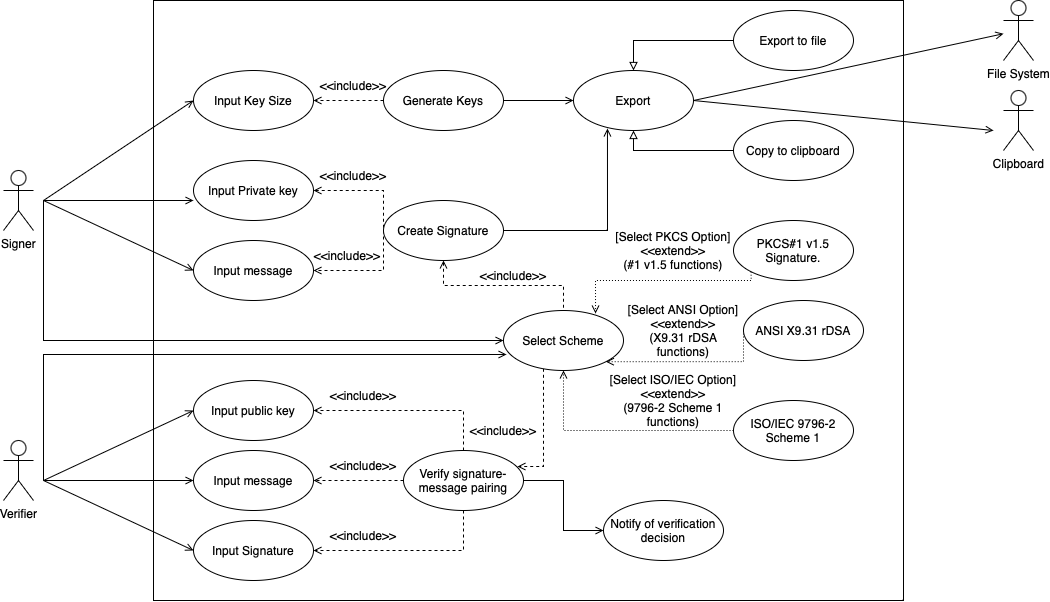
\includegraphics[scale=0.48]{POC_USE-CASE.png}
    \caption{UML Use Case Diagram}
    \label{fig:uc}
\end{figure}

Please see Appendix A for a description of the involved actors, a full breakdown of relevant requirements (capturing essential behaviour), and a flow-of-events type description for figure \ref{fig:uc} representing completed UML use cases, derived from preceding user stories.

\section{Key Generation}
\subsection{Design}
\begin{figure}[H]
    \centering
    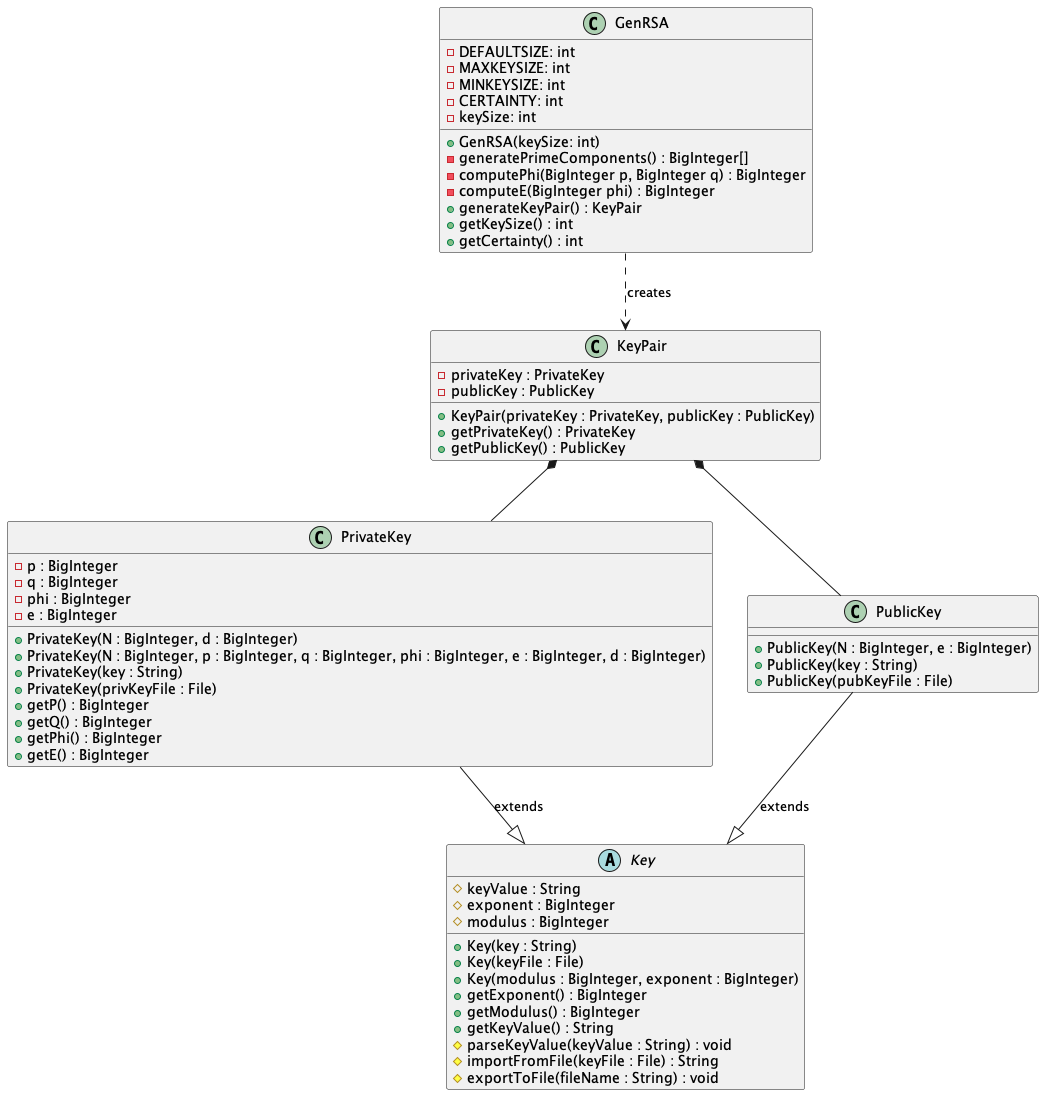
\includegraphics[scale=0.48]{KeyGeneration.png}
    \caption{Key Generation Class Design}
    \label{fig:kg}
\end{figure}

Figure \ref{fig:kg} provides a conceptualised design view of the foundational GenRSA definition discussed in section  \ref{subSec:keygen} aiming to act as bridge to implementation. The process is broken down into smaller components corresponding to roles/entities supportive to the purpose of generating keys. 


\begin{table}[H]
    \centering
    \caption{GenRSA Design}
    \label{tab:actors_description}
    \begin{tabular}{|l|p{10cm}|}
    \hline
    \textbf{Class} & \textbf{Description} \\
    \hline
    KeyGenRSA & Central class responsible for generating the key pair by providing a method to fulfil the generation process. \\
    \hline
    Key & Abstract class that serves as a blueprint for the public and private keys, encapsulating the use of the modulus and an accompanying exponent with further the ability to import/export its content. \\
    \hline
    PrivateKey / PublicKey & These classes extend from Key, specialising it for private and public key functionalities respectively. \\
    \hline
    \end{tabular}
\end{table}

\subsection{Implementation}
I opted to use Java for implementation detail. Particularly, its BigInteger class is well-suited for RSA due to its design. In practice it can handle arbitrarily long integers, provides essential arithmetic operations on these integers, and offers RSA-specific methods. It is not only a mature library having existed since Java 1.1 (year 1997) and thus likely to be well-tested/reliable but also actively supported and maintained. Given the relation to security this is a critical admission. 


This becomes immediately apparent when considering the generation of the large primes required to encompass N.
By employing the constructor BigInteger(int bitLength, int certainty, Random rnd), probable prime numbers of arbitrary value can be generated provided a certainty value is specified. 
\begin{lstlisting}[caption=Prime Generation with BigInteger]
public BigInteger[] generatePrimeComponents() {
    int adjustedBitLength = (int) Math.ceil(((double) keySize) / 2);
    BigInteger p = new BigInteger(adjustedBitLength, this.certainty, new SecureRandom());
    BigInteger q = new BigInteger(adjustedBitLength, this.certainty, new SecureRandom());
    return new BigInteger[]{p, q};
}
\end{lstlisting}
As with any RSA implementation the first step is initialising the RSA primes. 
Due to the magnitude of the integers in question, attempting to factorise both p and q to establish their primality with absolute certainty is computationally impractical. Instead, BigInteger employs the Miller-Rabin primality test to assess the probability of primality based on the probability of \[ 1 - \frac{1}{2^{certainty}}\]
For production-level security a value in the range 50-100 is the norm. I opted for the midpoint as a happy medium.

\begin{lstlisting}[caption=Key components]
  public BigInteger computePhi(BigInteger p, BigInteger q) {
    return p.subtract(ONE).multiply(q.subtract(ONE));
  }
  
  public BigInteger computeE(BigInteger phi) {
    BigInteger e = new BigInteger(phi.bitLength(), new SecureRandom());
    while (e.compareTo(ONE) <= 0 || !phi.gcd(e).equals(ONE) || e.compareTo(phi) >= 0) {
      e = new BigInteger(phi.bitLength(), new SecureRandom());
    }
    return e;
  }
\end{lstlisting}
The public key, \( e \), should belong to the group \( (Z/\phi Z)^{\times} \). To achieve this, a (positive) random \texttt{BigInteger} with the same number of bits as \( \phi \) is generated until a value from the group is identified. The \texttt{BigInteger} bitCount() method provides the means for doing this by returning the non-sign bit count of $\varphi$. 

The remaining computation in the attempt to obtain the private exponent d is straightforward with a naturally supported modInverse operation.
\begin{lstlisting}[caption=Java Implementation of Key Generation (\ref{subSec:keygen})]
  
  public KeyPair generateKeyPair() {
    BigInteger[] pq = this.generatePrimeComponents();
    BigInteger p = pq[0];
    BigInteger q = pq[1];
    BigInteger N = p.multiply(q);
    BigInteger phi = computePhi(p, q);
    BigInteger e = computeE(phi);
    BigInteger d = e.modInverse(phi);

    PublicKey publicKey = new PublicKey(N, e);
    PrivateKey privateKey = new PrivateKey(N, p, q, phi, e, d);

    return new KeyPair(publicKey, privateKey);
  }

\end{lstlisting}

\section{Design}


\begin{landscape}
\thispagestyle{lscape} % Apply the custom page style
\begin{figure}[H]
    \centering
    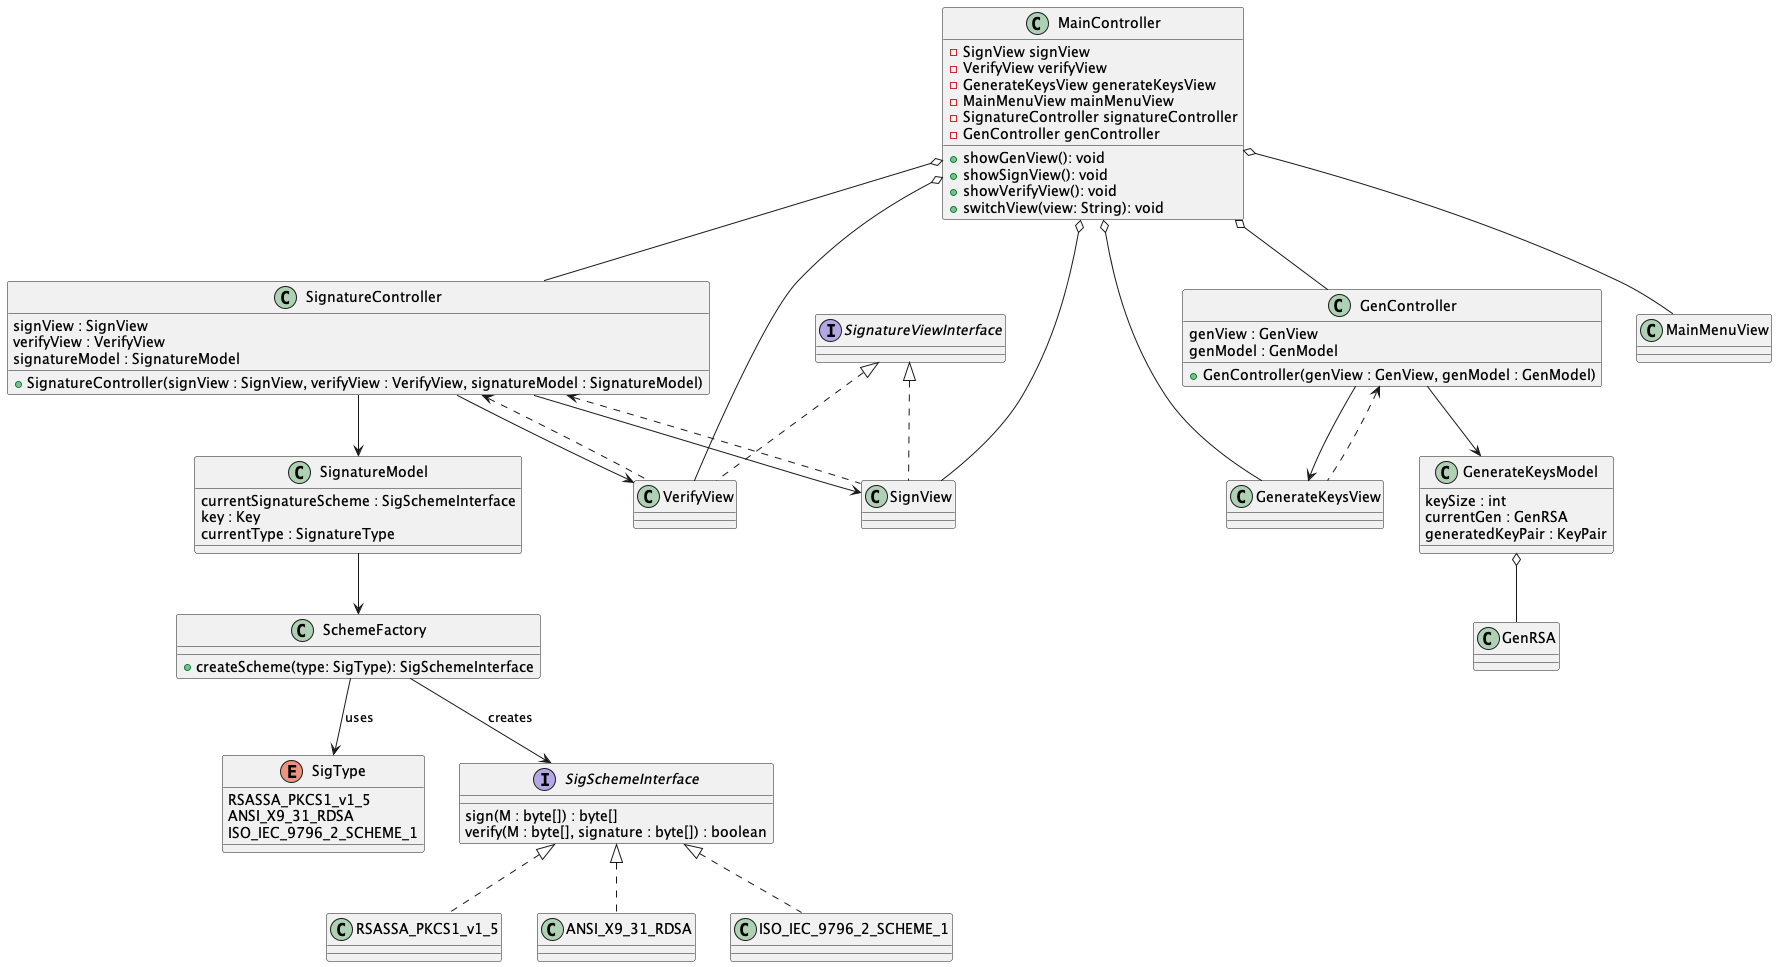
\includegraphics[width=\linewidth,keepaspectratio]{POC.png}
    \caption{POC program Class Design}
    \label{fig:POCCLASSES}
\end{figure}
\end{landscape}
Figure \ref{fig:POCCLASSES} depicts the structure of classes to be used in the implementation of the PoC program.  There is a focus on separation of concerns following the Model-View-Controller (MVC) design pattern. At the heart of the deign is the MainController, which orchestrates the application flow by responding to user actions and coordinating the display of different views. In support is the SignatureController, which manages the signature processes, linking the signature-related views (SignView and VerifyView) with the SignatureModel. SignatureModel encapsulates the cryptographic logic and relies on a SchemeFactory to instantiate a concrete signature scheme as per user selection. The system is further extended by the GenController which isfocused on generating cryptographic keys through the GenerateKeysModel which manages the GenRSA facilitated key creation.
\begin{figure}[H]
    \centering
    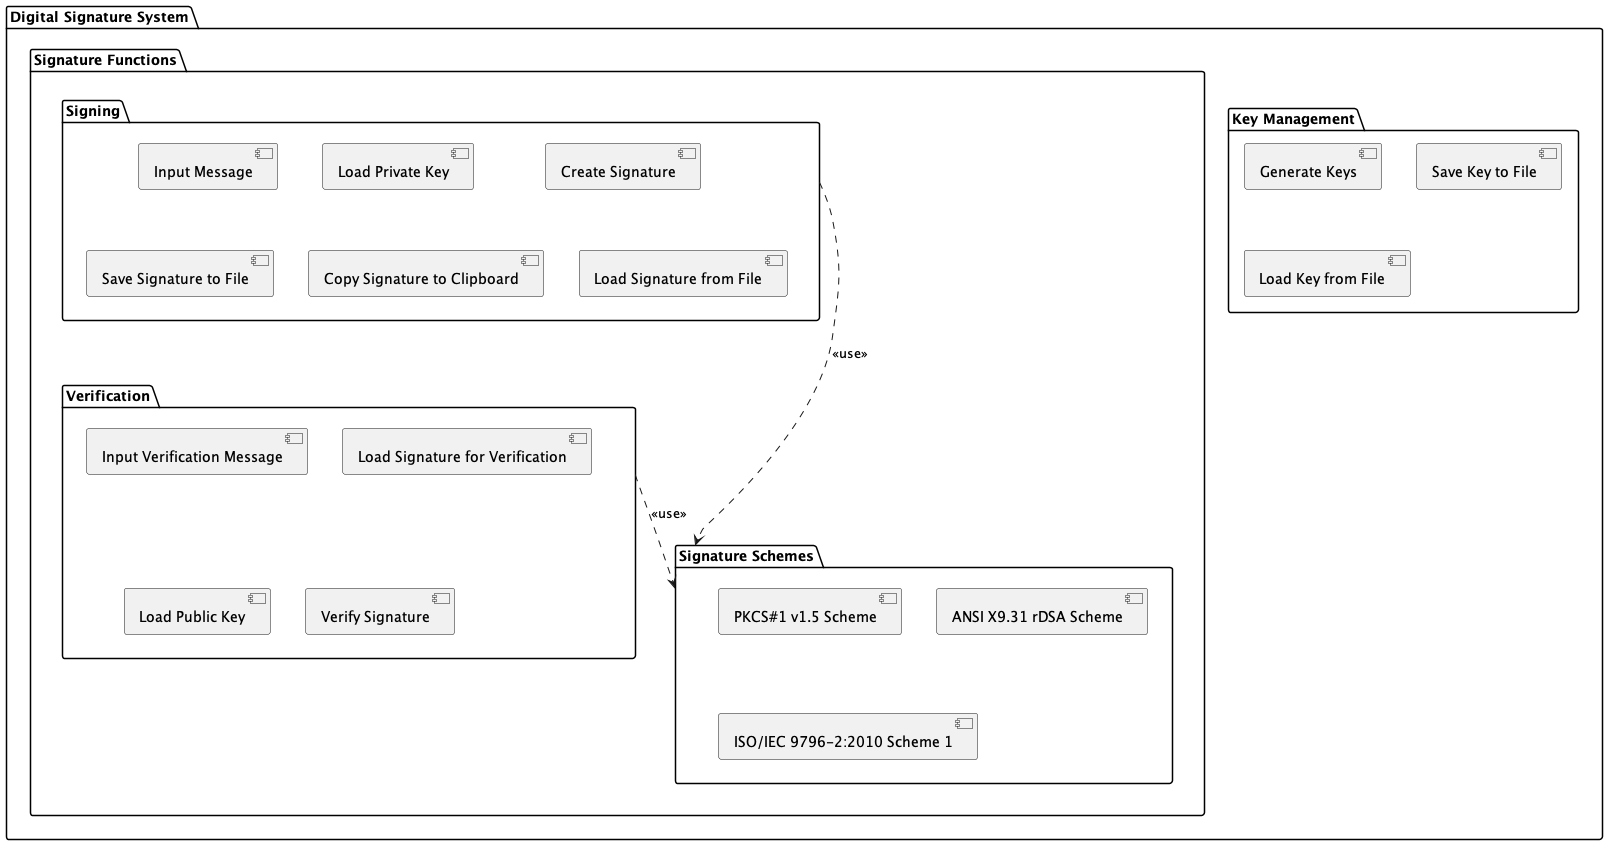
\includegraphics[scale=0.31]{package.png}
    \caption{POC program Packages}
    \label{fig:pack}
\end{figure}
Figure \ref{fig:pack} depicts the core functionality of the POC program and is in direct alignment with previously elaborated on (see requirements) user activities of signing, creating keys, and verifying, using a specified scheme like PKCS\#1-v1.5.



\chapter{Security Proofs}
Due to the breakthrough in 2018 \cite{jager2018security} when a security proof was provided for RSASSA-PKCS1-v1.5. It is possible to formally prove the security of the full class of deterministic RSA signatures. The precise statement of security is if the RSA problem is hard when H is modelled as a random oracle, then the scheme is secure (with regards to the UF-CMA notion i.e., full existential unforgeability against adaptive chosen message attacks). There are two different proofs for this, both which consider case where the modulus $\widehat{N}$ is a product of three primes. The first is based on the RSA assumption, the second is based on the $\phi$-Hiding assumption.


\section{Encode Algorithm}


Jager, Kakvi and May overcame the difficulty of providing proof for PKCS with a specialised encode algorithm that allows the simulation of signatures in polynomial time.  

\begin{definition}
Let
\[
(\widehat{y}, s, z) \xleftarrow{\$} \text{Encode}(N, e, y, \ell, \text{PAD}, R)
\]
be an efficient algorithm that takes as input an \(n\)-bit integer \(N\), an exponent \(e\), \(y \in \mathbb{Z}_N^*\), a hash value length $\ell$, padding pattern PAD and an \(r\)-bit prime \(R \in \mathbb{P}[r]\), and outputs \((\widehat{y}, s, z) \in \mathbb{Z}_{\widehat{N}} \times \mathbb{Z}_N^* \times \{0, 1\}^\ell\) or failure \(\bot\). \

\end{definition}

The algorithm outputs \((\widehat{y}, s, z)\) such that \(\widehat{y}\) has to be correct form for a PKCS\#1 signature mod \(\widehat{N}\) where \(z\) constitutes message hash and \(s\) comprises an \(e\)th root mod \(N\). Using this and the knowledge of \(R\) the \(e\)th root modulo \(\widehat{N}\) can be computed. More precisely it enables the encoding an arbitrary integer y modulo N as an integer $\hat{y}$ modulo $\hat{N} = NR$ for some prime R, such that $\hat{y}$ has correct PKCS\#1-V1.5 padding modulo $\hat{N}$.

\begin{enumerate}
\item y denotes an embedded RSA challenge that given a forgery can be solved i.e., obtaining \(\widehat{y} = PAD\|\|z \). 
\item In the case that \(y\) is replaced by 1 the algorithm instead stimulates a signature. 
\end{enumerate}
With these two uses of the Encode algorithm UF-CMA security of PKCS\#1 can be proved in the ROM. 

\begin{figure}[H]
\centering
\[
\boxed{
\begin{aligned}
&\underline{\textbf{Encode} (N, e, y, \ell, \text{PAD}, R)} \\
&n = \left\lceil \log_2 N \right\rceil, \; r = \left\lceil \log_2 R \right\rceil \\
&z := 2^\ell, \; k := 0 \\
&\textbf{while } (z \geq 2^\ell) \textbf{ and } (k < n \cdot 2^{-\ell}): \\
&\quad k := k + 1 \\
&\quad s \xleftarrow{\$} \mathbb{Z}_N \\
&\quad z := y^s e - 2^\ell \cdot \text{PAD} \mod N \\
&\quad \widehat{y} := 2^\ell \cdot \text{PAD} + z \\
&\textbf{if } z < 2^\ell \textbf{ then} \\
&\quad \textbf{return } (\widehat{y}, s, z) \\
&\textbf{else} \\
&\quad \textbf{return } \perp.
\end{aligned}
}
\]
\caption{Encode algorithm}
\label{fig:encode}
\end{figure}

The algorithm outputs \((\widehat{y}, s, z)\) except with negligible failure probability (in n). It can be said that encode efficiently $(n - \mathcal{O}(log \text{ } n))$-simulates the PKCS\#1 v1.5 encoding modulo $\hat{N} = NR$ which is true for a large hash value $\ell \approx |n|$.



\section{Background}
See section \ref{subSec:RSA-ASS} for the intuition behind trapdoor permutations in the context of its application to RSA.
\begin{definition}
\label{def:TDP}
A family of trapdoor permutations \( TDP = (\text{Gen}, \text{Eval}, \text{Invert}) \) comprises the following three polynomial-time algorithms:
\begin{enumerate}
    \item \textbf{Gen:} A probabilistic algorithm that, given input \( 1^k \), produces a public description \text{pub} (inclusive of an efficiently sampleable domain \( \text{Dom}_{\text{pub}} \)) and a trapdoor \( td \).
    
    \item \textbf{Eval:} A deterministic algorithm that, given \text{pub} and \( x \in \text{Dom}_{\text{pub}} \), yields \( y \in \text{Dom}_{\text{pub}} \). This relationship is expressed as \( f(x) = \text{Eval}(\text{pub}, x) \).
    
    \item \textbf{Invert:} A deterministic algorithm that, given \( td \) and \( y \in \text{Dom}_{\text{pub}} \), produces \( x \in \text{Dom}_{\text{pub}} \). This relationship is described by \( f^{-1}(y) = \text{Invert}(\text{pub}, y) \).
\end{enumerate}

It is required for all \( k \in \mathbb{N} \) and any (\text{pub}, td) produced by \(\text{Gen}(1^k)\):
\[ f(.) = \text{Eval}(\text{pub}, .) \text{ must define a permutation over } \text{Dom}_{\text{pub}} \]
and additionally for all \( x \in \text{Dom}_{\text{pub}} \):
\[ \text{Invert}(td, \text{Eval}(\text{pub}, x)) \text{ should equal } x \]

It's important to note that \( f_{\text{pub}}(.) = \text{Eval}(\text{pub}, .) \) needs to be a permutation for a correctly generated \text{pub}. 
\end{definition}

A trapdoor permutation is certified [5, 22] if one can publicly verify that it actually defines a permutation. 

\begin{definition} Certified Trapdoor permutation.
\label{def:CTDP}
A family of trapdoor permutations \( \text{TDP} \) is called \textit{certified} if there exists a deterministic polynomial-time algorithm \text{Certify} that, on input of \( 1^k \) and an arbitrary (polynomially bounded) bit-string \( \text{pub} \) (potentially not generated by \text{Gen}), returns 1 iff \( f(\cdot) = \text{Eval}(\text{pub}, \cdot) \) defines a permutation over \( \text{Dom}_{\text{pub}} \).
\end{definition}

Lossy Trapdoor Permutations are a realisation of the lossiness security notion for trapdoor permutations. Essentially, these permutations function in two distinct modes. The first allows for complete input recovery using an (injective) trapdoor function, while the second ((lossy) trapdoor function) causes substantial input data loss. Notably, distinguishing between these two behaviours is hard for any efficient adversary.

\begin{definition}
Let \( l \geq 2 \). A trapdoor permutation \( \text{TDP} \) is a \( (l, t, \varepsilon) \) lossy trapdoor permutation if the following two conditions hold:

\begin{enumerate}
    \item There exists a probabilistic polynomial-time algorithm \text{LossyGen}, which on input \( 1^k \) outputs \( \text{pub}' \) such that the range of \( f_{\text{pub}'}(\cdot) := \text{Eval}(\text{pub}', \cdot) \) under \( \text{Dom}_{\text{pub}'} \) is at least a factor of \( l \) smaller than the domain \( \text{Dom}_{\text{pub}'} \): 
    \[ |\text{Dom}_{\text{pub}'}|/|f_{\text{pub}'}(\text{Dom}_{\text{pub}'})| \geq l \]
    
    \item All distinguishers \( \mathcal{D} \) running in time at most \( t \) have an advantage \( \text{Adv}^L_{\text{TDP}}(\mathcal{D}) \) of at most \( \varepsilon \), where
    \[ \textbf{Adv}^L_{\text{TDP}}(\mathcal{D}) = \Pr[\textbf{L}_{1}^{\mathcal{D}}  \Rightarrow 1] - \Pr[\textbf{L}_{0}^{\mathcal{D}} \Rightarrow 1] \]
\end{enumerate}
\end{definition}

\begin{figure}[H]
\[
\boxed{
\begin{aligned}
&\underline{\textbf{\text{procedure Initialise Game } \(L_0\)}} \\
&(pub, td) \leftarrow_\$ \text{Gen}(1^k) \\
&\text{return } pub \\
\\
&\underline{\textbf{\text{procedure Initialise Game } \(L_1\)}} \\
&(pub', L) \leftarrow_\$ \text{LossyGen}(1^k) \\
&\text{return } pub' \\
\end{aligned}
}
\]
\caption{The Lossy Trapdoor Permutation Games.}
\label{fig:lossy_trapdoor_permutation_games}
\end{figure}

\begin{definition}
\label{def:reg-los}
\textit{Regular lossiness}. A TDP is regular \( (l, t, \varepsilon) \) lossy if the TDP is \( (l, t, \varepsilon) \) lossy and all functions \( f_{\text{pub}'}(\cdot) = \text{Eval}(\text{pub}', \cdot) \) generated by \text{LossyGen} are \( l \)-to-\( 1 \) on \( \text{Dom}_{\text{pub}'} \).
\end{definition}

\begin{definition} 
\textit{The RSA trapdoor permutation} \texttt{RSA} = (\texttt{RSAGen}, \texttt{RSAEval}, \texttt{RSAInv}): 
\begin{enumerate}
\item \texttt{RSAGen}($1^k$) outputs \texttt{pub} = (N,e) and \texttt{td} = d, where $N = pq$ is the product of two $k/2$-bit primes, \texttt{gcd}(e,$\phi(N)$) = 1, and $d = e^{-1} \mod \phi(N)$. 
\begin{itemize}
\item The domain is $\texttt{Dom}_{\texttt{pub}} = \mathbb{Z}_N^*$. 
\end{itemize}
\item \texttt{RSAEval}(\texttt{pub}, x) returns $f_{\texttt{pub}}(x) = x^e \mod N$, 
\item \texttt{RSAInv}(\texttt{td}, y) returns $f_{\texttt{pub}}^{-1}(y) = y^d \mod N$. 
\end{enumerate}

\end{definition} 

In the context of \texttt{RSA}, lossy trapdoor permutations can be viewed as the converse of certified trapdoor permutations. For example they entail an impossibility to differentiate an honestly generated (N, e) from (N, $e_{loss}$) for which $RSA_{N, e_{loss}}$ is many-to-1, thereby disqualifying themselves as permutations.


\subsection{2v3PA}
A final step computation assumption relevant to security statements in both proofs is the 2 vs 3 primes assumption \texttt{2v3PA}[$\lambda$]. It postulates that it's hard to discern if a specific modulus is derived from two or three prime factors. Although the assumption has never been formally studied it is widely accepted. Its role is to bridge the proofs to the setting of the typical two prime factor modulus.

\begin{definition}
\textit{The 2 vs. 3 Primes Assumption}. \texttt{2v3PA}[$\lambda$] states that it is hard to distinguish between $N_2$ and $N_3$, where $N_2$, $N_3$ are $\lambda$-bit numbers, where 
\begin{enumerate}
\item $N_2 = p_1 p_2$ is the product of 2 distinct random prime numbers $p_1, p_2 \in \mathbb{P}$; 
\item $N_3 = q_1 q_2 q_3$ is the product of 3 distinct random prime numbers $q_1, q_2, q_3 \in \mathbb{P}$
\end{enumerate}
\texttt{2v3PA}[$\lambda$] is said to be $(t, \epsilon)$-hard, if for all distinguishers $\mathcal{D}$ running in time at most $t$, we have:
\[
\textbf{Adv}^{\texttt{2v3PA}[\lambda]}_\mathcal{D} = \Pr[1 \leftarrow \mathcal{D}(N_2)] - \Pr[1 \leftarrow \mathcal{D}(N_3)] \leqslant \epsilon
\]
\end{definition}

\section{Security Proof under the RSA Assumption}
The computation assumption relevant to security statements in the first proof is the RSA Assumption \text{k-}\texttt{RSA}[$\lambda$] (See definition \ref{def:RSA-ASS}).

\section{Security Proof under the Phi-Hiding Assumption}
The computation assumption relevant to security statements in the second proof is the $\varphi$-Hiding Assumption k-$\phi$HA[$\lambda$]. 
It posits that for a given modulus \( N \) and a sufficiently small exponent \( e \) (\( e < N^{\frac{1}{4}} \)), determining if \(\frac{e}{\phi(N)}\) is hard. 

By definition \ref{def:reg-los} when gcd(\( \hat{e}_{\text{loss}} \),\( \phi(N) \)) = \( \hat{e}_{\text{loss}} \) the $RSA_{N, \hat{e}_{loss}}$ function is \( \hat{e}_{loss}{\text{-to-}}1 \) i.e., \( \hat{e}_{\text{loss}}- \)regular lossy.

\begin{definition}
\textit{The $\varphi$-Hiding Assumption}. K-$\phi$HA[$\lambda$], states that it is hard to distinguish between $(N,e_{inj})$ and $(N,\hat{e}_{loss})$, where 
\begin{enumerate}
\item $N$ is a $\lambda$-bit number and is the product of k distinct random prime numbers $p_i \in \mathbb{P}[n_i]$, for $i \in \llbracket1, \ldots, k \rrbracket$, $k$ constant, and $\displaystyle\sum_{i=1}^{n} n_i = n$ 
\item $e_{inj}, \hat{e}_{loss} > 3 \in \mathbb{P}$;
\item $e_{inj}, \hat{e}_{loss} \leq N^{1/4}$, with $\gcd(e_{inj}, \varphi(N)) = 1$ and $\gcd(\hat{e}_{loss}, \varphi(N)) = \hat{e}_{loss}$, where $\varphi$ is the Euler Totient function. 
\end{enumerate}
k-$\phi$\texttt{HA}[$\lambda$] is said to be $(t, \epsilon)$-hard, if for all distinguishers $\mathcal{D}$ running in time at most $t$, we have:
\[
\textbf{Adv}^{\text{k-}\phi \texttt{HA}[\lambda]}_\mathcal{D} = \Pr[1 \leftarrow D(N, e_{inj})] - \Pr[1 \leftarrow D(N,\hat{e}_{loss})] \leqslant \epsilon
\]
\end{definition}






%%%% ADD YOUR BIBLIOGRAPHY HERE
\newpage

\addcontentsline{toc}{chapter}{Bibliography}
\printbibliography
\label{endpage}
\end{document}

\end{article}
